\documentclass{scrartcl}[10pt,a4paper]

\usepackage[T1]{fontenc}
\usepackage{lmodern}
%\usepackage{csquotes} %useful for quoted text (with command \enquote)
\usepackage{xspace}
\usepackage{microtype}
\usepackage[bookmarks,bookmarksopen,bookmarksdepth=2]{hyperref}
\usepackage{graphicx}
\usepackage[style=numeric,backend=bibtex8]{biblatex}

\addbibresource{bibliography.bib}
%\usepackage{makeidx}

%\makeindex

%Bugfix for BibTeX
\makeatletter
\def\blx@maxline{77}
\makeatother

\begin{document}

\newcommand\myemojiname{My emoji\xspace}
\newcommand\myemoji{\raisebox{-.4ex}{\protect
\includegraphics[height=2.5ex]{proposed_e000.png}}}

\title{Emoji Submission: \MakeUppercase{\myemojiname} \\ \myemoji}
%\date{\today}
\author{John Doe}

\maketitle
\tableofcontents

    \section{Proposal for New Emoji}

    \section{Names}
        \subsection{CLDR short name}
        Recommended name: \MakeUppercase{\myemojiname}
        \subsection{CLDR keywords}
        Recommended keywords:
    \section{Images}
    \section{Selection Factors -- Inclusion}
        \subsection{Compatibility}
        \subsection{Expected usage level}
            \paragraph{Frequency}
            Because of the numerous different meanings of a \myemojiname character ({\myemoji}), a high usage level is expected.
            \begin{figure}[b]
				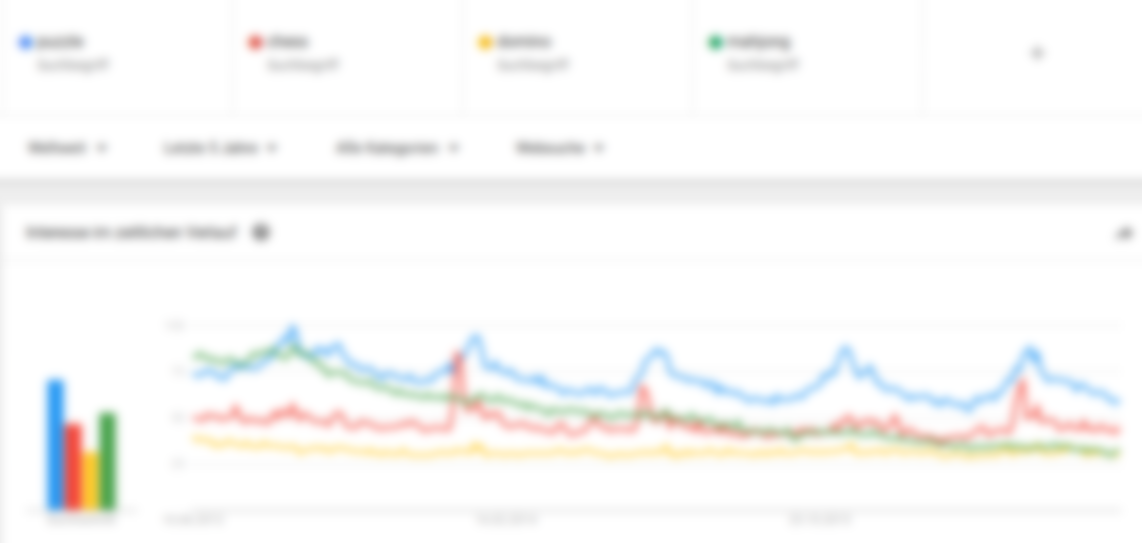
\includegraphics[width=1\textwidth]{google_trends.png}
				\caption{Google Trends, \textit{\myemojiname} compared to other popular games}
				\label{fig:trends}
				\end{figure}
				In figure \ref{fig:trends} you see a comparsion of the usage of the term \textit{puzzle} and \textit{Lorem Ipsum}.
            \paragraph{Multiple usages}
            \paragraph{Use in Sequences}
        \subsection{Image distinctiveness}
        \subsection{Completeness}        
        \subsection{Frequently requested}
        \begin{figure}[b]
				
\includegraphics[width=.5\textwidth]{twitter1.png}
				
\includegraphics[width=.5\textwidth]{twitter2.png}
				
\includegraphics[width=.5\textwidth]{twitter3.png}
				
\includegraphics[width=.5\textwidth]{twitter4.png}
				\caption{Various Twitter users requesting a \textit{\myemojiname} emoji}
				\label{fig:twitter}
        \end{figure}
        
        Figure \ref{fig:twitter} shows a selection of Twitter users who are requesting a \textit{\myemojiname} emoji. Also see \cite{exam} for further reference.
    \section{Selection Factors -- Exclusion}
        \subsection{Overly specific}
        \subsection{Open-ended}
        \subsection{Already Representable}
        \subsection{Logos, brands, UI icons, signage, specific people, deities}     
        \subsection{Transient}
        \subsection{Faulty Comparison}
    \section{Sort location}
        \subsection{Category}
        Recommended category:
        \subsection{Emoji before}
        Recommended emoji before: xxxx (U+XXXX)
    \section{Other Information}
    
    \printbibliography

%\printindex

\end{document}